\documentclass[11pt,letterpaper]{article}
\usepackage[utf8]{inputenc}
\usepackage[T1]{fontenc}
\usepackage[margin=1in]{geometry}
\usepackage{amsmath,amssymb}
\usepackage{graphicx}
\usepackage{hyperref}
\usepackage{xcolor}
\usepackage{enumitem}
\usepackage{caption}

\hypersetup{colorlinks=true,linkcolor=black,urlcolor=black,citecolor=black}
\graphicspath{{../figures/}}

\title{\textbf{Zoo Gaming Mechanics}\\\large Tamagotchi-Style Pet Care Meets Game-Fi}
\author{Antje Worring \\ \textit{Founder, Zoo Labs Foundation} \\ \texttt{antje@zoo.ngo}}
\date{October 31, 2021}

\begin{document}
\maketitle

\begin{abstract}
This element paper expands the gaming mechanics from the Zoo Whitepaper~\cite{zoo2021}. Zoo's gameplay weaves Tamagotchi-style pet care --- feed, grow, breed --- with collateralization, daily yield, and a generation-limited breeding curve. We document the lifecycle, the egg drop mechanics, the boost ladder, and the play-and-earn games that anchor user engagement.
\end{abstract}

\section{The lifecycle}

A Zoo animal proceeds through four stages:

\begin{enumerate}
  \item \textbf{Egg.} Acquired in a drop. Three rarity tiers: Sublime (1 ETH, 5\%), Rare (0.5 ETH, 15\%), Endangered (0.05--0.1 ETH, 85\%).
  \item \textbf{Baby.} Hatching is free. The baby earns the lowest tier of daily reward.
  \item \textbf{Teen.} Minted by feeding the NFT 1$\times$ the original egg price (OEP). The teen earns a higher daily reward.
  \item \textbf{Adult.} Minted by feeding 2$\times$ OEP. The adult earns the highest daily reward and unlocks breeding.
\end{enumerate}

Adults of the same species can be bred to mint a new egg for 3$\times$ OEP, which goes to the DAO rather than as staked collateral.

\section{The pre-drop whitelist}

Before each drop, users on the whitelist can purchase one random egg --- of any rarity tier --- for the price of the most common egg. This means a whitelisted user might pay 0.05 ETH and discover they own a Sublime egg worth 1 ETH. This drop mechanic incentivizes early community participation without requiring users to gamble on rarity tiers.

\section{The boost ladder}

Daily rewards are amplified by a boost multiplier keyed to the dollar value of staked collateral:

\begin{itemize}
  \item \$10--\$99: 1.1$\times$.
  \item \$100--\$999: 1.2$\times$.
  \item \$1{,}000--\$9{,}999: 1.3$\times$.
  \item \$10{,}000+: 1.4$\times$.
\end{itemize}

The yield formula is \emph{daily reward} $+$ (\emph{collateral} $\times$ \emph{boost} $\times$ \emph{days/365}). The Zoo Reward Calculator surfaces projected earnings.

\section{The breeding curve}

Each egg generation has a one-baby/one-teen/one-adult mint limit. Adult animals with breeding privileges can breed with another adult of the same species to mint the next generation egg. The breeding-allowance curve descends:

\begin{itemize}
  \item Gen 1: 7 allowances.
  \item Gen 2: 6.
  \item Gen 3: 5.
  \item Gen 4: 4.
  \item Gen 5: 3.
  \item Gen 6: 2.
  \item Gen 7: 0.
\end{itemize}

Adults can be sold with or without remaining breeding privileges. This curve enforces scarcity.

\section{Daily reward schedule by rarity}

\begin{itemize}
  \item \textbf{Sublime}: Baby 1 \$ZOO; Teen 2 \$ZOO; Adult 3 \$ZOO.
  \item \textbf{Rare}: Baby 0.25 \$ZOO; Teen 0.5 \$ZOO; Adult 1 \$ZOO.
  \item \textbf{Endangered}: Baby 0.05 \$ZOO; Teen 0.1 \$ZOO; Adult 0.2 \$ZOO.
\end{itemize}

A Sublime adult earns 60$\times$ the daily reward of an Endangered baby. The reward asymmetry reflects the rarity asymmetry.

\section{Play-and-earn games}

Two flagship mini-games:

\paragraph{Coin Runner.} An endless-runner mechanic. Player dashes through a temple collecting gold/silver coins of escalating denomination, ending in a bullion bar. All rewards redeemable for physical precious metals.

\paragraph{Memory Bridge.} A pattern-memory mechanic. Player crosses a bridge in 4 seconds per level by stepping on the correct brick. Bridge lengthens as levels progress.

Both games surface the Lux Token (gold/silver-backed) as the rewards substrate, tying gameplay rewards to commodity-backed value.

\section{Asset transfer}

Two ways to extract NFT value:

\begin{enumerate}
  \item \textbf{Marketplace sale.} Sell at a price exceeding purchase + collateral + accrued rewards. Buyer inherits all collateral, accrued rewards, and breeding privileges.
  \item \textbf{Burn.} Destroys the NFT and refunds collateral + accrued rewards, minus the 20\% sustainability tax (10\% DAO, 10\% liquidity pool).
\end{enumerate}

Burning ends the lineage of that NFT permanently, removing it from circulation.

\section{Why this is durable gameplay}

The Zoo gameplay loop is durable because every action surfaces at least one of: economic upside, conservation impact, or emotional bond. There is no purely speculative move. Even burning --- which seems extractive --- routes 10\% to the DAO conservation treasury. Even breeding --- which seems like dilution --- pays the 3$\times$ OEP fee to the DAO.

\begin{figure}[h]
\centering
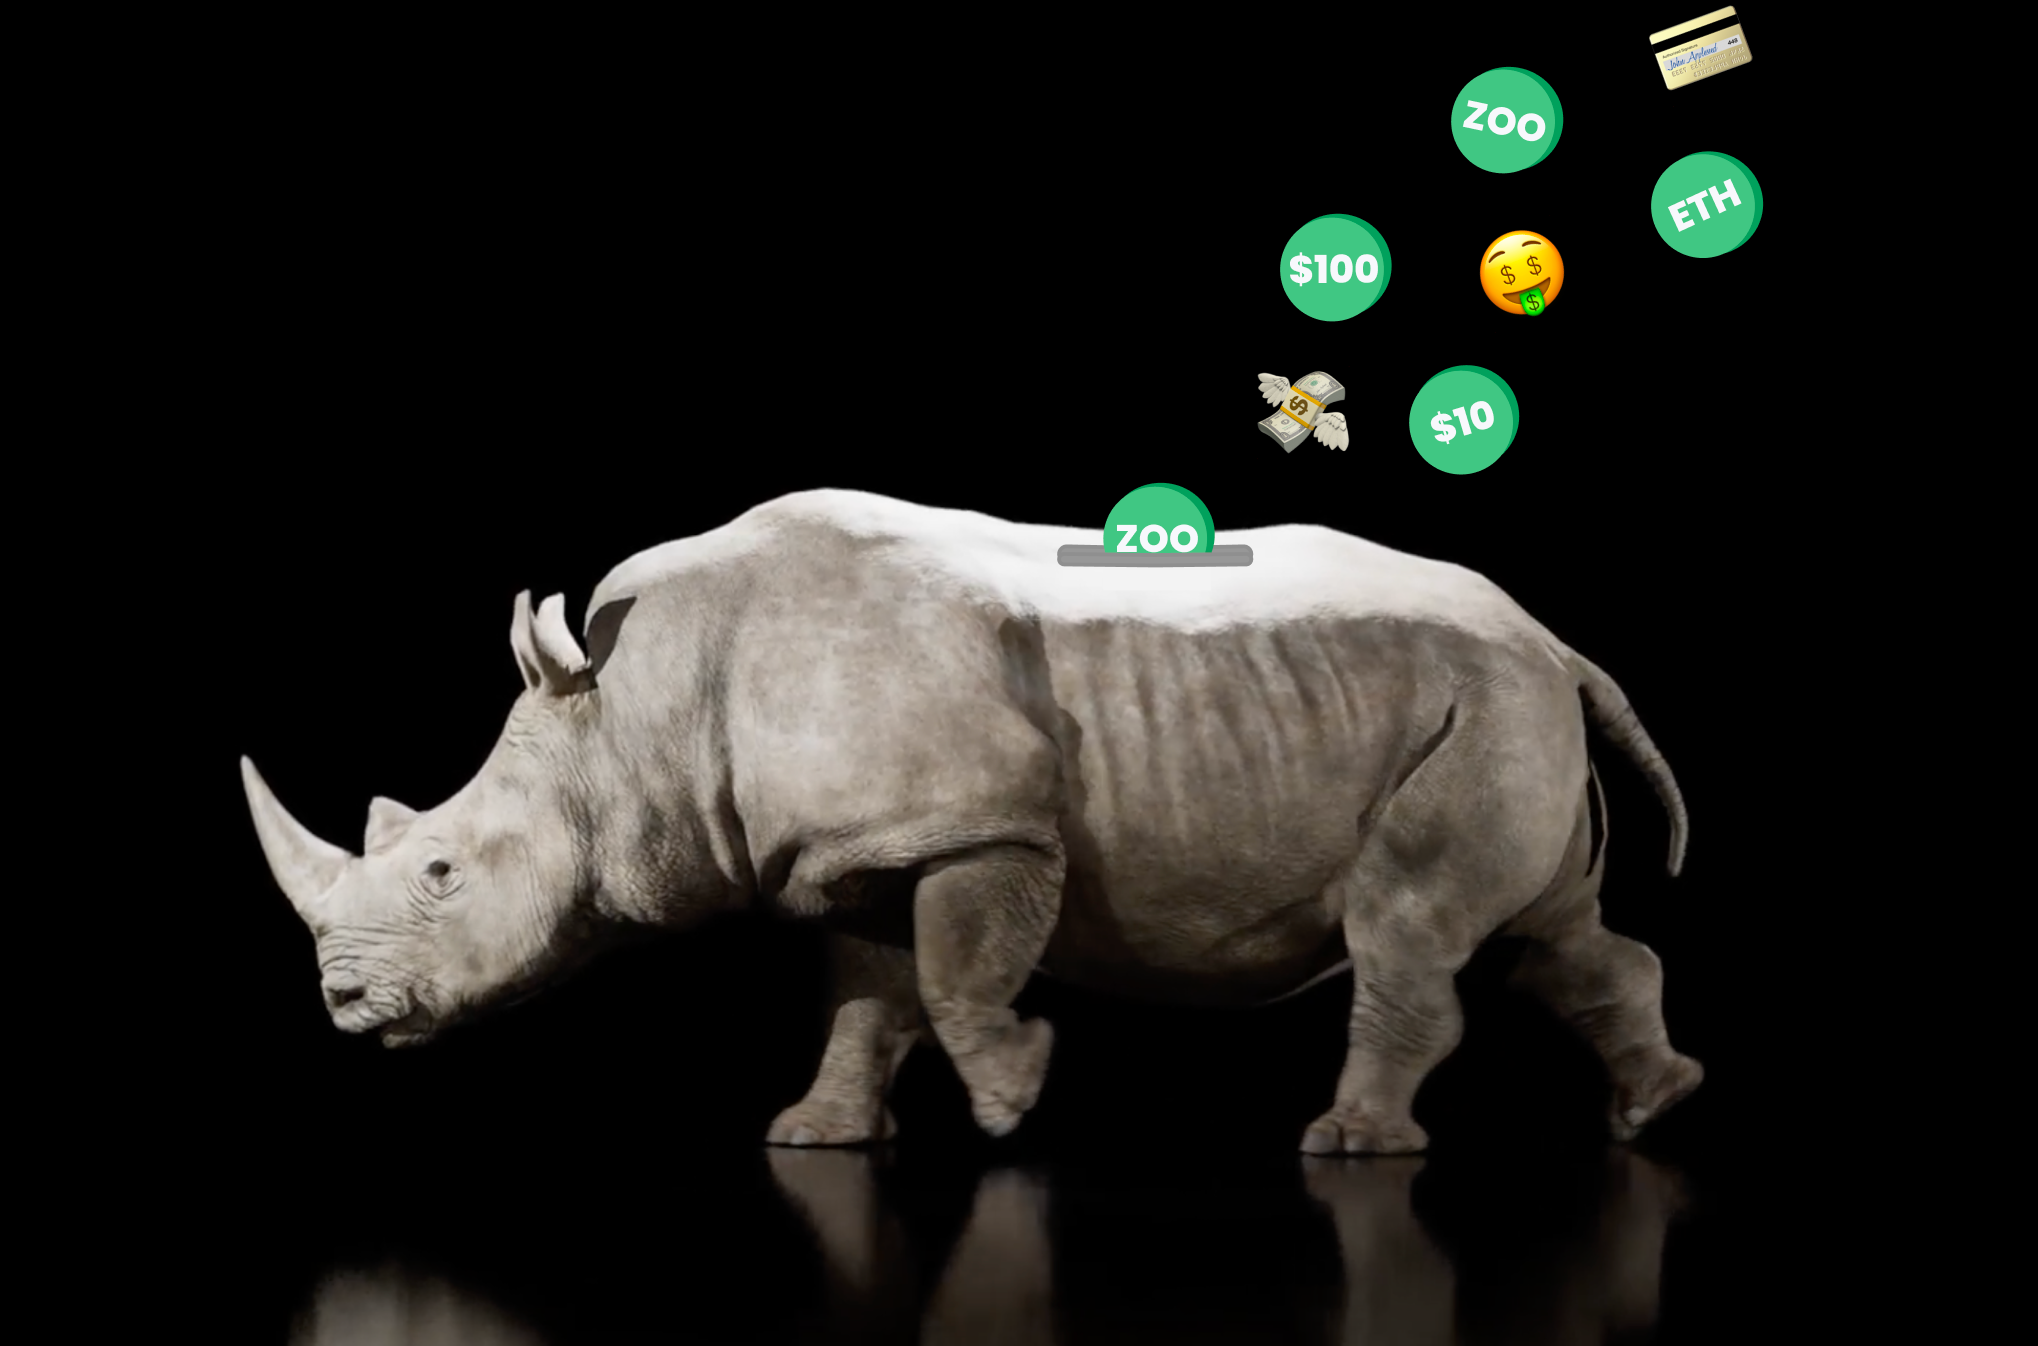
\includegraphics[width=0.55\textwidth]{collateral.png}
\caption{Collateral diagram. Feeding an animal stakes value into its NFT, which then earns boosted daily rewards proportional to the staked amount.}
\end{figure}

\section{Pools}

Beyond single-NFT trades, holders can group multiple NFTs into a \emph{pool} listed at a single set price. The buyer pays the pool price (in any cryptocurrency or fiat, converted to \$ZOO under the hood) and atomically receives every NFT in the pool, along with all collateral and accrued rewards. Pools accelerate liquidity for collectors who want to exit a curated collection.

\section{Marketplace UX commitments}

Per~\cite{zoo2021}, the Zoo Marketplace commits to:

\begin{itemize}
  \item Crypto and credit/debit-card payment paths in a single seamless checkout.
  \item Sellers are paid in their listed currency regardless of how the buyer paid.
  \item Direct \$ZOO purchases via card to lower the on-ramp barrier for new entrants.
  \item Asset Transfer flow that hands over NFT \emph{plus its stored value} in one transaction.
  \item Leaderboard surfacing top NFTs and top users by cumulative collection value.
\end{itemize}

These choices reflect a deliberate stance: Zoo wants to onboard the gaming demographic, not only the existing crypto-native demographic.

\section{Marketplace fees}

Listing and selling on the Zoo Market is \textbf{free}. The fees that apply are:

\begin{itemize}
  \item \textbf{Royalty (2.5\%)} --- charged on every sale or mint, paid to the original creator.
  \item \textbf{Hatching} --- free; effectively burns the egg and mints the baby.
  \item \textbf{Mint Teen} --- 1$\times$ original egg price (OEP), staked into the NFT.
  \item \textbf{Mint Adult} --- 2$\times$ OEP, staked.
  \item \textbf{Breeding} --- 3$\times$ OEP, paid to the DAO (not staked).
\end{itemize}

\section{Sustainability tax breakdown}

The whitepaper~\cite{zoo2021} specifies the following tax schedule:

\begin{itemize}
  \item \textbf{\$ZOO Liquidity Pool Tax (8\%)}: 4\% to LP, 4\% to DAO. Applied on every sell.
  \item \textbf{KEEPER Liquidity Pool Tax (8\%)}: 4\% to LP, 4\% to DAO. Applied on every sell.
  \item \textbf{NFT Burn Tax (20\%)}: 10\% to LP, 10\% to DAO. Applied when collateral-backed NFT is liquidated via burn.
\end{itemize}

These splits are designed to keep liquidity pools healthy while building the conservation treasury.

\begin{thebibliography}{1}
\bibitem{zoo2021} Antje Worring. \emph{Zoo: A Game-Fi Multiverse Ecosystem for the Preservation of Endangered Species}. Zoo Labs Foundation, October 31, 2021.
\end{thebibliography}

\end{document}
